\DiaryEntry{Inside Interesting Integrals, Feynman's Trick (Chap 3), II}{2022-04-05}{Integrals}

\subsection{Sinc-Integral}

We start with

\bee
g(y) = \int_0^\infty e^{-xy} \frac{\sin ax}{x} dx, \quad y > 0
\eee

with some constant $a$. Let's differentiate wrt parameter $y$ to obtain

\bee
\frac{dg}{dy} = \int_0^\infty (-x) e^{-xy} \frac{\sin ax}{x} dx = - \int_0^\infty e^{-xy} \sin ax dx
\eee

This is a "standard" integral known to be

\bee
\int_0^\infty e^{-xy} \sin ax dx = \frac{a}{a^2 + y^2}
\eee

and we can now integrate $\frac{dg}{dy} = - \frac{a}{a^2 + y^2}$ to obtain

\bee
g(y) = C - \arctan \left(\frac{a}{y}\right)
\eee

The integration constant $C$ can be obtained by observing that $g(y) = \int_0^\infty e^{-xy} \frac{\sin ax}{x} dx$ goes to zero for $y \rightarrow \infty$ (because in the ntegration interval $x > 0$ and therefore the exp-function vanishes). Therefore,

\bee
0 = C - \tan (\pm \infty) \rightarrow C = \pm \frac{\pi}{2}
\eee

with the $\pm$ according to the sign of $a$. Therefore,

\bee
\boxed{
g(y) = \int_0^\infty e^{-xy} \frac{\sin ax}{x} dx = \sign(a) \left(\frac{\pi}{2}\right) - \arctan \left(\frac{y}{a} \right)
}
\eee

We can check this result with Maxima.

\begin{verbatim}
    (%i54)	a:3;y:2;
    (%o53)	3
    (%o54)	2
    (%i55)	f:exp(-x*y)*sin(a*x)/x;
    (%o55)	(%e^(-2*x)*sin(3*x))/x
    (%i56)	quad_qags(f, x, 0, 1000);
    (%o56)	[0.982793723247329,5.523470466813409*10^-11,357,0]
    (%i57)	%pi/2 - atan(y/a), numer;
    (%o57)	0.982793723247329
\end{verbatim}


For the special case of $g(0) = \int_0^\infty \frac{\sin ax}{x} dx$, we obtain

\be\label{2022-04-05:eq2}
\int_0^\infty \frac{\sin ax}{x} dx = \begin{cases} \frac{\pi}{2}, \quad a > 0 \\
    0, \quad a = 0 \\
    -\frac{\pi}{2}, \quad a < 0
    \end{cases} \qed
\ee

As an aside, let's calculate the "standard" integral

\bee
I =\int_0^\infty e^{-ax} \sin bx dx
\eee

We perform integration by parts with $u = e^{-ax}, v' = \sin(bx)$ and $u'=(-a)e^{-ax}, v = - 1/b \cos(bx)$ and obtain

\bee
I = - \left. \frac{1}{b} e^{-ax} \cos(bx) \right|_0^\infty  - \int_0^\infty (-a)e^{-ax} \left( -\frac{1}{b} \right) \cos(bx) dx = \frac{1}{b} - \frac{a}{b} \int_0^\infty e^{-ax} \cos(bx) dx
\eee

It seems as if we have not gained anything; however, we see that application of integration by parts "converted" the initial sine into a cosine. Let's do this again\dots

We chose $u = e^{-ax}, v' = \cos(bx)$ and $u'=(-a)e^{-ax}, v = 1/b \cos(bx)$ and get

\bee
I = \frac{1}{b} - \frac{a}{b} \left( \left. \frac{1}{b} e^{-ax} \sin(bx) \right|_0^\infty - \int_0^\infty (-a)e^{-ax} \frac{1}{b} \sin(bx) dx \right)
\eee

which can be further evaluated into

\bee
I = \frac{1}{b} - \frac{a^2}{b^2} \int_0^\infty e^{-ax} \sin(bx) dx
\eee

That looks better; let's write down what we have

\bee
\int_0^\infty e^{-xy} \sin ax dx = \frac{1}{b} - \frac{a^2}{b^2} \int_0^\infty e^{-ax} \sin(bx) dx
\eee

from which we obtain

\bee
\left( \int_0^\infty e^{-xy} \sin ax dx \right) \left(1 +  \frac{a^2}{b^2} \right) = \frac{1}{b}
\eee

and finally

\bee
\boxed{
    \int_0^\infty e^{-ax} \sin bx dx =  \frac{b}{a^2 + b^2}
} \qed
\eee

The integrand is shown in the following Figure; not overly exciting: $a$ controls the exponential decay, $b$ the oscillation frequency.

\begin{figure}[H]
    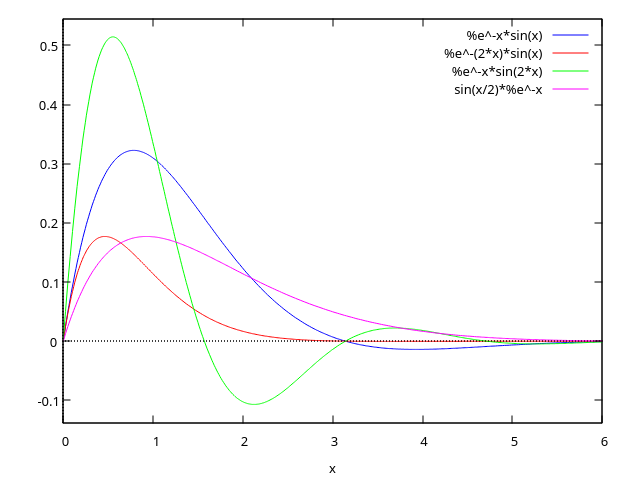
\includegraphics[scale=0.7]{images/2022-04-05_plot_1.png}
\end{figure}

The dependence of the integral value $\frac{b}{a^2 + b^2}$ on the oscillation frequency $b$ is interesting: It has a peak at $b = a$. Slow and fast oscillations yield a smaller integral value: Slow oscillations cause the exponential decay to kick in, dampening the curve; fast oscillation contain a negative area reducing the area under the curve.

The integral value for $a = 1$ as function of $b$ is shown in the following Figure.

\begin{figure}[H]
    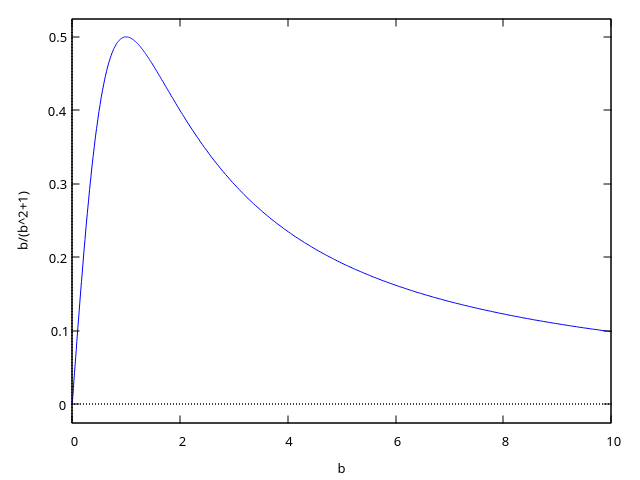
\includegraphics[scale=0.7]{images/2022-04-05_plot_2.png}
\end{figure}


\subsection{Frullani's Integral}

We consider the integral

\bee
I(a,b) = \int_0^\infty \frac{\arctan(ax) - \arctan(bx)}{x} dx
\eee

We can integrate wrt $a$ to obtain

\begin{align*}
  \frac{\partial I(a,b)}{\partial a} &= \int_0^\infty \frac{1}{x} \frac{\partial }{\partial a} \arctan ax dx = \int_0^\infty \frac{1}{x} \frac{x}{1+a^2 x^2} dx = \int_0^\infty \frac{1}{1+a^2 x^2} dx = \\
  &= \frac{1}{a} \left. \arctan \frac{x}{a} \right|_0^\infty = \frac{\pi}{2a}
\end{align*}

We integrate wrt $a$ to obtain

\bee
I(a,b) = \frac{\pi}{2} \log a + C(b)
\eee

where $C(b)$ is the constant of integration (constant wrt $a$, however a function wrt $b$). We can do whatever we want with $C(b)$; to get it inside the log, we write $\frac{\pi}{2}\log C(b)$ and get


\be\label{2022-04-05:eq1}
I(a,b) = \frac{\pi}{2} \log a + \frac{\pi}{2}\log C(b) = \frac{\pi}{2} \log(a C(b))
\ee

The special case $a = b$ yields $I(a,a) = 0$ and we obtain

\bee
I(a,a) = 0 = \frac{\pi}{2} \log(a C(a)) \rightarrow \log(a C(a)) = 0 \rightarrow a C(a) = 1 \rightarrow C(a) = \frac{1}{a}
\eee

Inserting the value back into \eqref{2022-04-05:eq1}, we obtain

\bee
I(a,b) = \frac{\pi}{2} \log \left( a \frac{1}{b} \right) = \frac{\pi}{2} \log \left( \frac{a}{b} \right)
\eee

and the integral becomes

\bee
\boxed{
  I(a,b) = \int_0^\infty \frac{\arctan(ax) - \arctan(bx)}{x} dx =  \frac{\pi}{2} \log \left( \frac{a}{b} \right)
  }
\eee

The integrand is shown in the following Figure for different values of $a$. If $a < b$, the plot is mirrored at the $x$-axis (and the integral becomes negative).

\begin{figure}[H]
    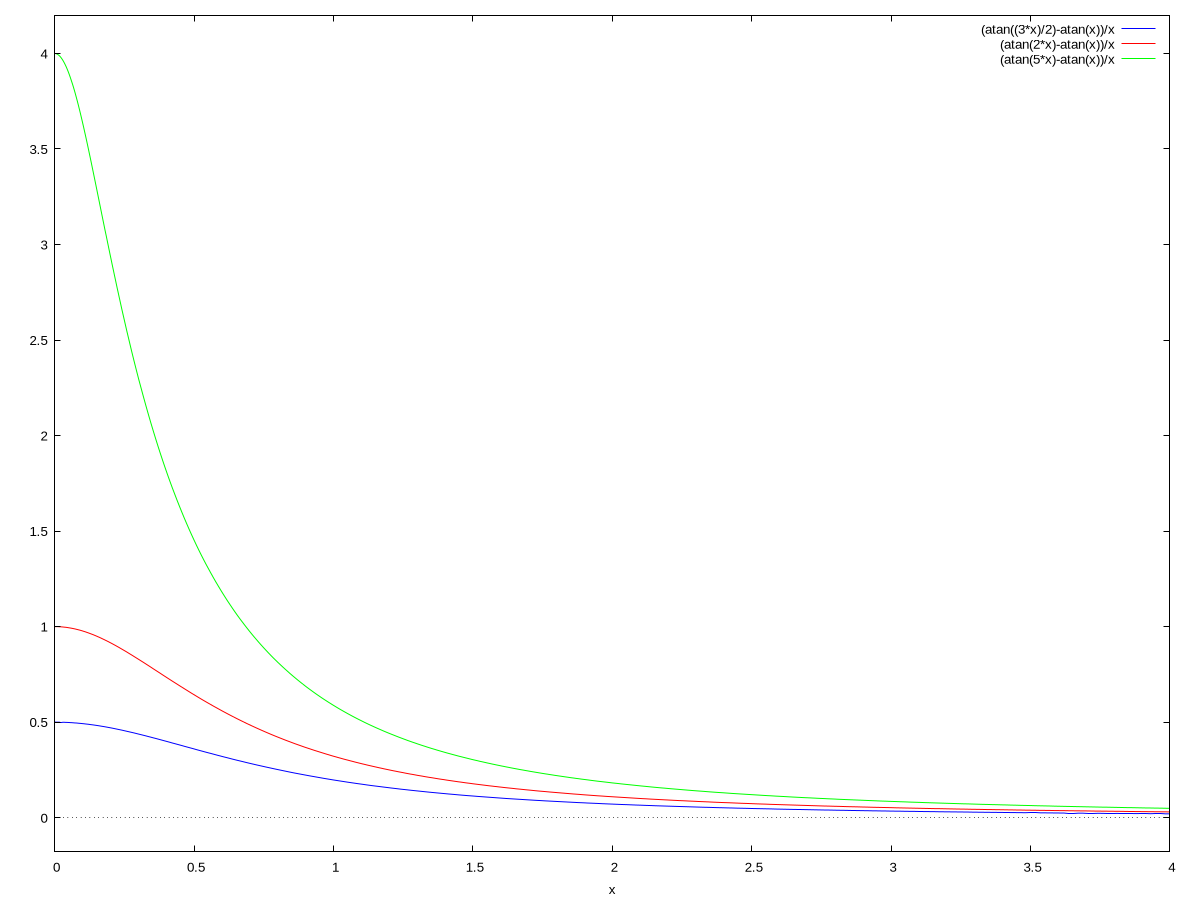
\includegraphics[scale=0.3]{images/2022-04-05_plot_3.png}
\end{figure}

The integral we just did can be generalized to any function $f(x)$ as long as $f(0)$ and $f(\infty)$ exist. We define an integral

\bee
U = \int_0^{h/a} \frac{f(ax) - f(0)}{x} dx
\eee

with some positive constant $h$. We can split the integral and rearrange expressions to arrive at

\bee
U = \int_0^{h/a} \frac{f(ax)}{x} dx - f(0) \int_0^{h/a} \frac{1}{x} dx \rightarrow \int_0^{h/a} \frac{f(ax)}{x} dx = U + f(0) \int_0^{h/a} \frac{1}{x} dx
\eee

We can simply replace $a$ with $b$ and get

\bee
\int_0^{h/b} \frac{f(bx)}{x} dx = U + f(0) \int_0^{h/b} \frac{1}{x} dx
\eee

Let's subtract the two equations; we have

\begin{align*}
  \int_0^{h/a} \frac{f(ax)}{x} dx - \int_0^{h/b} \frac{f(bx)}{x} dx &= U + f(0) \int_0^{h/a} \frac{1}{x} dx - U - f(0) \int_0^{h/b} \frac{1}{x} dx \\
                                                                    &= f(0) \int_0^{h/a} \frac{1}{x} dx - f(0) \int_0^{h/b} \frac{1}{x} dx \\
                                                                    &= f(0) \left( \log(x)|_0^{h/a} - \log(x)|_0^{h/b} \right) = f(0) log \frac{\frac{h}{a}}{\frac{h}{b}} \\
                                                                    &= f(0) \log \frac{b}{a}
\end{align*}

Next we sneak in a term $\int_{h/b}^{h/a} \frac{f(bx)}{x} dx$ and obtain

\bee
\int_0^{h/a} \frac{f(ax)}{x} dx - \int_0^{h/b} \frac{f(bx)}{x} dx - \int_{h/b}^{h/a} \frac{f(bx)}{x} dx + \int_{h/b}^{h/a} \frac{f(bx)}{x} dx = f(0) \log \frac{b}{a}
\eee

We can combine the second and third term into one integral,

\bee
\int_0^{h/a} \frac{f(ax)}{x} dx - \int_0^{h/a} \frac{f(bx)}{x} dx + \int_{h/b}^{h/a} \frac{f(bx)}{x} dx = f(0) \log \frac{b}{a}
\eee

and combine the integrands of the first and second term,

\bee
\int_0^{h/a} \frac{f(ax) - f(bx)}{x} dx + \int_{h/b}^{h/a} \frac{f(bx)}{x} dx = f(0) \log \frac{b}{a}
\eee

Now we take the limit $h \rightarrow \infty$. The first integral is easy as it becomes an integral from $0$ to $\infty$. The second integral is a bit trickier: Both integration boundaries
go to $\infty$ and we can therefore argue that $f(bx) \rightarrow f(\infty)$ over the integration range and move it as a constant before the integral. So we have

\bee
\lim_{h \rightarrow \infty} \int_{h/b}^{h/a} \frac{f(bx)}{x} dx = \lim_{h \rightarrow \infty} f(h) \int_{h/b}^{h/a} \frac{1}{x} dx =  \lim_{h \rightarrow \infty} f(h) \left. \log(x) \right|_{h/b}^{h/a} = f(\infty) \log \frac{b}{a}
\eee

We therefore have the result

\bee
\boxed{
  \int_0^\infty \frac{f(ax) - f(bx)}{x} dx = \left( f(0) - f(\infty) \right) \log \left( \frac{b}{a} \right)
}
\eee

Be careful; this works only when both limits $f(0), f(\infty)$ are defined as is the case with $\arctan$ (above) or $\exp$ as in

\bee
  \int_0^\infty \frac{e^{-ax} - e^{-bx}}{x} dx = \left( 1 - 0 \right) \log \left( \frac{b}{a} \right) = \log \left( \frac{b}{a} \right)
\eee

We can demonstrate this via numpy

\begin{verbatim}
import numpy as np
import scipy.integrate as int

def f(x):
    val = (np.exp(-x) - np.exp(-2*x))/x
    return(val)

inte.quad(f, 0, 1000)
>>> (0.6931471805599451, 2.009305447347239e-11)

np.log(2/1)
>>> 0.6931471805599453
\end{verbatim}


%%% Local Variables:
%%% mode: latex
%%% TeX-master: "journal"
%%% End:
